% state diagrams
%
The major goal of this report is to develop a real-world application. In order to do this, all real-world implications need to be taken into consideration. There are certain states in which the system can reside depending on its own battery state, the battery state of neighbour nodes and the availability of a energy bar or energy checkpoint. These states and their transmissions are displayed in figure \ref{fig:states}. The battery can either be sufficiently full $V_{full}$, in starving state $V_{starve}$ or in a depleted state $V_{dead}$. These parameters are further specified in section \ref{sec:proposed}. With help of the state diagram we can write protocols to accomodate the state changes. The figure displays a composed state called capable. This state encapsulates the behavior of the product whenever it is capable of doing something functional such as charging and running a show. 

\begin{figure}[h!]
\centering
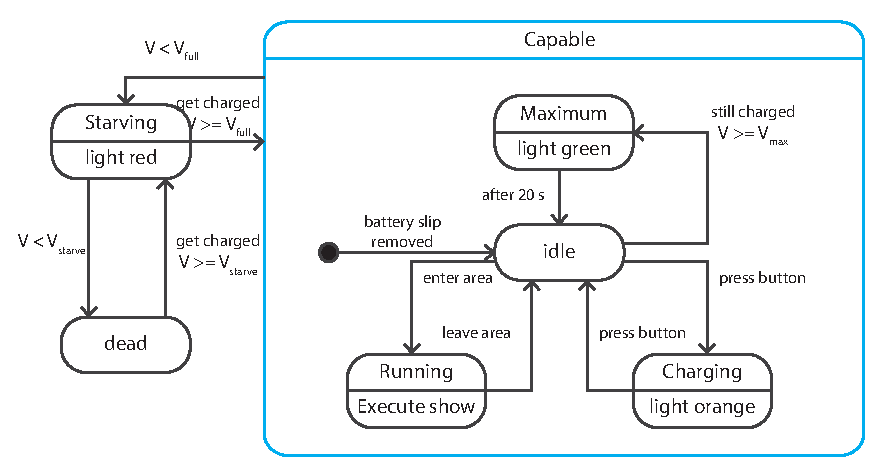
\includegraphics[width=0.8\textwidth]{statediagram.pdf}
\caption{State diagram of a transceiving wireless power transfer system}
\label{fig:states}
\end{figure}

Whilst creating this state diagram we created several insights that introduced new features into the system:
\begin{itemize}
	\item The need for a charge actuator. A button is added for the user to determine when to charge another user as we don't want to constantly send energy. 
	\item An indication of $V_{max}$. The user needs to know when charging does not have any effect anymore. We will use a red light to indicate $V_{max}$ is being reached. 
	\item Indicate the charging. To give the user a complete insight in the working principles of the system a blinked orange indicator is added whenever a wristband is receiving charge to indicate the wireless transfer is working properly. 
\end{itemize}

